\documentclass[12pt,english]{article}
\usepackage[a4paper,bindingoffset=0.2in,%T
            left=1in,right=1in,top=1in,bottom=1in,%
            footskip=.25in]{geometry}
\usepackage{blindtext}
\usepackage{caption}
\usepackage{subcaption}
\usepackage{titling}
\usepackage{amssymb}
\usepackage{amsmath}
\usepackage{listings}
\usepackage{lettrine} 
\usepackage{tikz}  
\usepackage{color}
\setlength{\parskip}{12pt}
\begin{document}
\newgeometry{left=0.8in,right=0.8in,top=1in,bottom=1in}
\begin{center}
    \Large
    \textbf{Homework 2}\\
    \small
    \today\\
    \large
    Jose Carlos Munoz
\end{center}
%===============================
\section*{1}
\begin{align*}
H(a,b) &= 4\\
H(a,c) &= 3
\end{align*}
String a and c are the most similar becuase they have the lowest hamming distance.
\section*{2}
$\alpha$ has a total of 10 elements.
$\beta$ has a total of 11 element.
$\lambda$ has a total of 12 element.
\begin{align*}
J(\alpha, \beta) = \frac{\alpha\cap\beta}{\alpha\cup\beta} =
\frac{7}{14} = .5 & &
J(\alpha, \lambda) = \frac{\alpha\cap\lambda}{\alpha\cup\lambda} =
\frac{8}{14} = .571
\end{align*}
$\alpha$ and $\lambda$ are the most similar because they have the highest Jaccard coefficient.
\section*{3}
\begin{align*}
E(human, animal) &= 4\\
E(human, plant) &= 4
\end{align*}
Both animal and plant have the same similarity to human because their edit distance is 4 for each.
\section*{4}
$\vec{X}*\vec{Y} = 1 * 0 + 2 * 2 + 2 * 0 = 4$.
$\vec{X}*\vec{Z} = 1 * -2 + 2 * 2 + 2 * -1 = 0$
\begin{align*}
\mid \vec{X} \mid &= \sqrt(1^2 + 2^2 + 2^2) &=\sqrt(1 + 4 + 4 ) &=\sqrt(9) &= 3\\
\mid \vec{Y} \mid &= \sqrt(0^2 + 2^2 + 0^2) &=\sqrt(0 + 4 + 0 ) &=\sqrt(4) &= 2\\
\mid Z \mid &= \sqrt(-2^2 + 2^2 + -1^2) &=\sqrt(4 + 4 + 1 ) &=\sqrt(9) &= 3
\end{align*}
$S_C(X,Y) = \frac{4}{3 * 2} = \frac{2}{3}$.
$S_C(X,Z) = \frac{0}{3 * 3} = \frac{0}{9}$.
Vector Y is the most similar to Vector Z. This is becuase the cosine value of $S_C(X,Y)$ is much greater than $S_C(X,Z)$
\section*{5} 
\begin{figure}[!h]
\centering
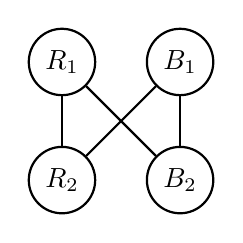
\begin{tikzpicture}[node distance={15mm}, thick, main/.style = {draw, circle}] 
\node[main] (1) {$R_1$}; 
\node[main] (2) [below of=1] {$R_2$}; 
\node[main] (3) [right of=1] {$B_1$};
\node[main] (4) [right of=2] {$B_2$};
\draw(1) -- (2);
\draw(1) -- (4);
\draw(2) -- (3);
\draw(3) -- (4);
\end{tikzpicture} 
\end{figure}
The figure above has a modularity of 0. This is because the $Q_R$ and $Q_B$ are the same. The calculation for both is \\
\begin{align*}
Q_{(R,B)} &= \frac{1}{4} - \left( \frac{2+2}{2 * 4}\right)^2\\
Q_{(R,B)} &= \frac{1}{4} - \left( \frac{1}{2} \right)^2\\
Q_{(R,B)} &= \frac{1}{4} - \left( \frac{1}{4} \right)\\
Q_{(R,B)} &= 0\\
\end{align*}
Adding all of these Q, we get that the modularity of the network is 0
\section*{6}
\begin{figure}[!h]
\centering
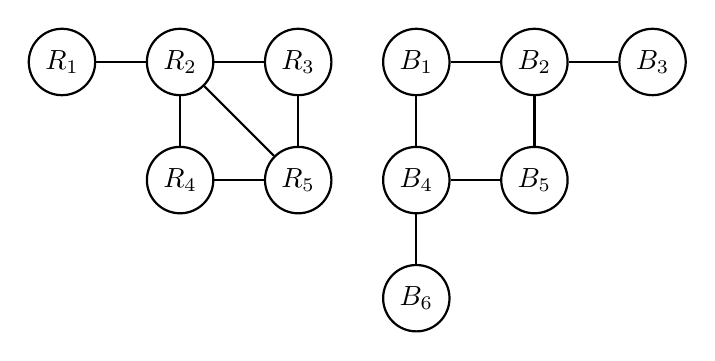
\begin{tikzpicture}[node distance={15mm}, thick, main/.style = {draw, circle}] 
\node[main] (1) {$R_1$}; 
\node[main] (2) [right of=1] {$R_2$}; 
\node[main] (3) [right of=2] {$R_3$};
\node[main] (4) [below of=2] {$R_4$};
\node[main] (5) [right of=4] {$R_5$};
\node[main] (6) [right of=3] {$B_1$}; 
\node[main] (7) [right of=6] {$B_2$}; 
\node[main] (8) [right of=7] {$B_3$};
\node[main] (9) [below of=6] {$B_4$};
\node[main] (10) [below of=7] {$B_5$};
\node[main] (11) [below of=9] {$B_6$};
\draw(1) -- (2);
\draw(2) -- (3);
\draw(2) -- (4);
\draw(2) -- (5);
\draw(3) -- (5);
\draw(4) -- (5);

\draw(6) -- (7);
\draw(7) -- (8);
\draw(6) -- (9);
\draw(7) -- (10);
\draw(9) -- (10);
\draw(9) -- (11);
\end{tikzpicture} 
\end{figure}
The figure above has a modularity of 0.5. The calculation for both is \\
\begin{align*}
Q_{(R)} &= \frac{6}{12} - \left( \frac{1 +2+2+3+4}{2 * 12}\right)^2 & &Q_{(B)} &= \frac{6}{12} - \left( \frac{1+3+2+2+3+1}{2 * 12}\right)^2\\
Q_{(R)} &= \frac{6}{12} - \left( \frac{12}{2 * 12}\right)^2 & &Q_{(B)} &= \frac{6}{12} - \left( \frac{12}{2 * 12}\right)^2\\
Q_{(R)} &= \frac{1}{2} - \left( \frac{1}{2}\right)^2 & &Q_{(B)} &= \frac{1}{2} - \left( \frac{1}{2}\right)^2\\
Q_{(R)} &= \frac{1}{2} - \frac{1}{4} & &Q_{(B)} &= \frac{1}{2} - \frac{1}{4}\\
Q_{(R)} &= \frac{1}{4} & &Q_{(B)} &= \frac{1}{4}
\end{align*}
Adding all of these Q, we get that the modularity of the network is 0.5
\end{document}